\documentclass[10pt, a4paper, titlepage]{article}

\usepackage[T2A]{fontenc}
\usepackage[utf8]{inputenc}
\usepackage[russian]{babel}

\usepackage{hyperref}
\hypersetup{pdftitle={Методология проектирования структур данных. Индивидуальное задание. Разработка модели данных зоологической коллекции}, pdfauthor={Верхотуров В.С.}, colorlinks=false, pdfborder={0 0 0}}

\usepackage{authblk} % affilations on the titlepage

\usepackage{graphicx}

\usepackage{float} % Вставить картинку в определенное место

\title{Методология проектирования структур данных. Индивидуальное задание. Разработка модели данных зоологической коллекции}
\author{Верхотуров В.С.}
\affil{БСБО-05-20}
\affil{РТУ МИРЭА}
\date\today


\begin{document}

\maketitle

\tableofcontents
\newpage

\section{Анализ предметной области}

\subsection{Общая характеристика}

Зоологические коллекции (фондовые научные коллекции зоологических институтов, университетов, музеев, а также собрания чучел, препаратов и частей объектов животного мира, живые коллекции зоопарков, зоосадов, цирков, питомников, аквариумов, океанариумов и других учреждений), представляющие научную, культурно-просветительную, учебно-воспитательную и эстетическую ценность, отдельные выдающиеся коллекционные экспонаты независимо от формы их собственности подлежат государственному учету.

\subsection{Организационная структура}
\label{sec:organizationalStructure}

Порядок государственного учета, пополнения, хранения, приобретения, продажи, пересылки, вывоза за пределы Российской Федерации и ввоза в нее зоологических коллекций или отдельных экспонатов определяет уполномоченный Правительством Российской Федерации федеральный орган исполнительной власти.

Государственный учет зоологических коллекций в Российской Федерации осуществляется Государственным комитетом Российской Федерации по охране окружающей среды (Госкомэкология России) путем ведения государственного реестра.

Юридические лица и граждане, являющиеся владельцами таких коллекций и экспонатов, обязаны соблюдать порядок их учета, хранения, использования и пополнения.

\subsection{Функциональная структура}

Предоставление данных Госкомэкологии России для исполнения обязанности по соблюдению порядка учета зоологической коллекции, хранения, использования и пополнения.

\subsection{Характеристика документов}

\href{https://docs.cntd.ru/document/9011346}{\textbf{Федеральный закон от 24 апреля 1995 г. № 52-ФЗ "О животном мире"}}.

Закон содержит раздел <<Статья 29. Зоологические коллекции>>, описанный в \autoref{sec:organizationalStructure}.

Животный мир является достоянием народов Российской Федерации, неотъемлемым элементом природной среды и биологического разнообразия Земли, возобновляющимся природным ресурсом, важным регулирующим и стабилизирующим компонентом биосферы, всемерно охраняемым и рационально используемым для удовлетворения духовных и материальных потребностей граждан Российской Федерации.

\href{https://docs.cntd.ru/document/58812875}{\textbf{Приказ Госкомэкологии России от 30 сентября 1997 г. № 411 "О Положении о зоологических коллекциях" (Минюст N 1507 08.04.98)}}.

Содержание:
\begin{enumerate}
    \item Приказ <<О Положении о зоологических коллекциях>>;
    
    \item Положение о зоологических коллекциях;
    
    \item Форма реестра зоологических коллекций, поставленных на государственный учет;
    
    \item Форма свидетельства о внесении зоологической коллекции в реестр;
    
    \item Форма разрешения на вывоз за пределы Российской Федерации и ввоз на ее территорию зоологических коллекций, их частей и отдельных экспонатов.

\end{enumerate}

Во исполнение постановления \href{https://docs.cntd.ru/document/9026760?marker}{Правительства Российской Федерации от 17.07.96 N 823 "О порядке государственного учета, пополнения, хранения, приобретения, продажи, пересылки, вывоза за пределы Российской Федерации и ввоза на ее территорию зоологических коллекций"} и согласно \href{https://docs.cntd.ru/document/9050595?marker}{Постановлению Правительства Российской Федерации от 26.05.97 N 643 "Об утверждении Положения о Государственном комитете Российской Федерации по охране окружающей среды" (С3, 1997, N 22, ст.2605)}.


\section{Модель предметной области}

\subsection{Диаграмма модели предметной области типа <<Сущность -- связь>>}

\begin{figure}[H]
    \centering
    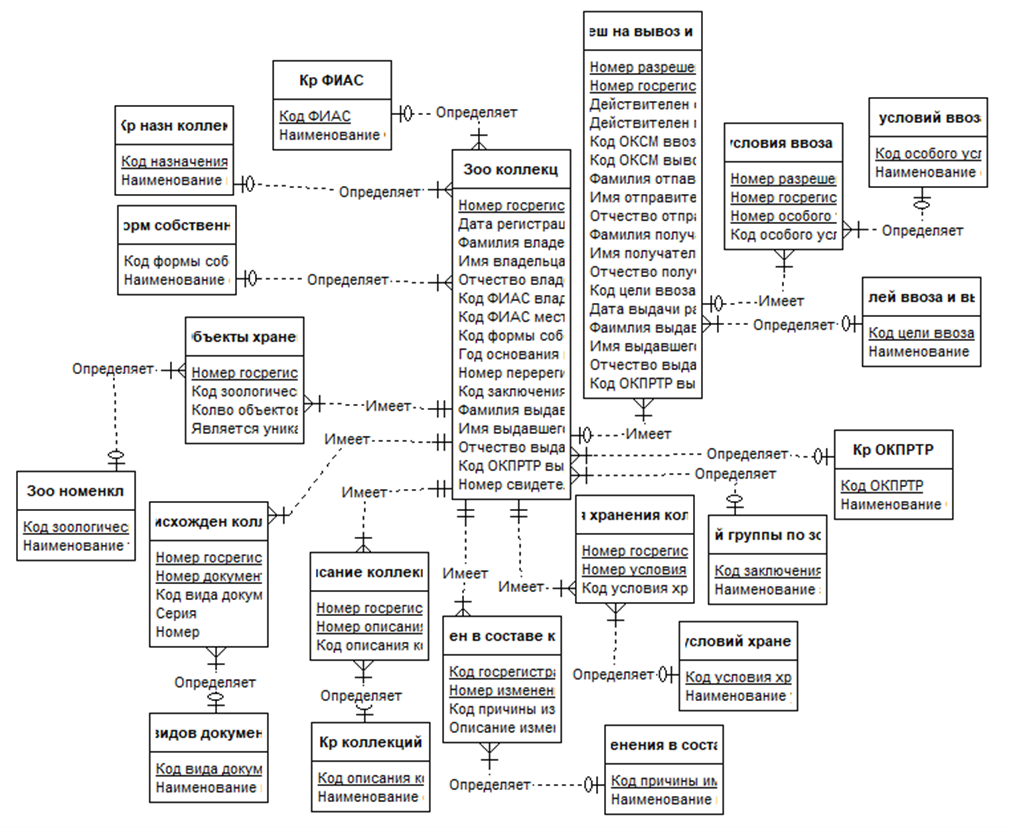
\includegraphics[height=9cm]{image.png}
    \caption{Диаграмма модели предметной области}
    \label{fig:er_diagram}
\end{figure}








\subsection{Спецификация модели предметной области}







\subsection{Нормализация схем сущностей}






\section{Реляционная модель данных}




\subsection{Получение реляционных отношений из модели предметной области}

{
    % Macros
    
    %% Keys
    
    %%% Primary Key
    \newcommand{\pk}[1]{\textbf{#1}}
    
    %%% Foreign Key
    \newcommand{\fk}[1]{\textit{#1}}
    
    %%% Primary Foreign Key
    \newcommand{\pfk}[1]{\pk{\fk{#1}}}
    
    %% Columns
    \newcommand{\firstColumn}[4]{#1 - \newline #2 - \newline #3 \newline\newline #4}
    
    \newcommand{\thirdColumn}[6]{
    #1 \newline 
    \underline{Первичный ключ} - #2 \newline 
    \setbox0=\hbox{#3\unskip}\ifdim\wd0=0pt
    \else
      \underline{Внешний(е) ключ(-и)}: #3 \newline
    \fi
    #4 \newline 
    \underline{Первичный ключ} - #5 \newline
    \setbox0=\hbox{#6\unskip}\ifdim\wd0=0pt
    \else
      \underline{Внешний(е) ключ(-и)}: #6 \newline
    \fi
    }
    
    \newcommand\generalizedColumn[6]{\thirdColumn{#1:}{#2}{#3}{#4:}{#5}{#6}}
    
    
    %%  Rules
    
    %%% 1
    \newcommand\ruleOneMondatoryOneMondatoryNum{1}
    \newcommand\ruleOneMondatoryOneMondatory{1 Об - 1 Об}
    
    %%% 2
    \newcommand\ruleOneMondatoryOneOptionalNum{2}
    \newcommand\ruleOneMondatoryOneOptional{1 Об - 1 Н/О}
    \newcommand\ruleOneOptionalOneMondatoryNum{2}
    \newcommand\ruleOneOptionalOneMondatory{1 Н/О - 1 Об}
    
    %%% 3
    \newcommand\ruleOneOptionalOneOptionalNum{3}
    \newcommand\ruleOneOptionalOneOptional{1 Н/О - 1 Н/О}
    
    %%% 4
    \newcommand\ruleOneOptionalManyMondatoryNum{4}
    \newcommand\ruleOneOptionalManyMondatory{1 Н/О - М Об}
    \newcommand\ruleManyMondatoryOneOptionalNum{4}
    \newcommand\ruleManyMondatoryOneOptional{М Об - 1 Н/О}
    
    \newcommand\ruleOneMondatoryManyMondatoryNum{4}
    \newcommand\ruleOneMondatoryManyMondatory{1 Об - М Об}
    \newcommand\ruleManyMondatoryOneMondatoryNum{4}
    \newcommand\ruleManyMondatoryOneMondatory{М Об - 1 Об}
    
    %%% 5
    \newcommand\ruleOneMondatoryManyOptionalNum{5}
    \newcommand\ruleOneMondatoryManyOptional{1 Об - М Н/О}
    \newcommand\ruleManyOptionalOneMondatoryNum{5}
    \newcommand\ruleManyOptionalOneMondatory{М Н/О - 1 Об}
    
    \newcommand\ruleOneOptionalManyOptionalNum{5}
    \newcommand\ruleOneOptionalManyOptional{1 Н/О - М Н/О}
    \newcommand\ruleManyOptionalOneOptionalNum{5}
    \newcommand\ruleManyOptionalOneOptional{М Н/О - 1 Н/О}
    
    %%% 6
    \newcommand\ruleManyOptionalManyOptionalNum{6}
    \newcommand\ruleManyOptionalManyOptional{М Н/О - М Н/О}
    
    %% Entities
    
    \subsubsection{Таблица перехода}
    
    
    
    
    
    
    \subsubsection{Итоговые реляционные отношения}
    
    
    
    
}

\subsection{Нормализация реляционных отношений}



\subsection{Спецификация реляционной модели данных}



\end{document}
